\documentclass[12pt,a4paper,twoside,openright,usefrontespizio]{toptesi}

% --- Language and encoding ---
\usepackage[T1]{fontenc}
\usepackage[utf8]{inputenc}
\usepackage{lmodern}

% --- Layout ---
\usepackage{setspace}
\onehalfspacing
\raggedbottom

% --- Math and symbols ---
\usepackage{amsmath,amssymb}

% --- Graphics ---
\usepackage{graphicx}
\usepackage{float}

% --- Tables ---
\usepackage{booktabs}

% --- Code listings ---
\usepackage{xcolor}
\usepackage{listings}
\lstset{
  basicstyle=\ttfamily\small,
  breaklines=true,
  frame=single,
  columns=fullflexible
}

% --- References and links ---
\usepackage{hyperref}
\hypersetup{
    colorlinks=true,
    linkcolor=black,
    citecolor=black,
    urlcolor=black
}
\usepackage{bookmark}

% --- Quotes ---
\usepackage{csquotes}

% --- Bibliography ---
\usepackage[
    backend=biber,
    style=ieee
]{biblatex}
\addbibresource{bibliografia.bib}

% --- Custom commands ---
\newcommand{\ie}{i.e., }
\newcommand{\eg}{e.g., }
\newcommand{\etal}{et al. }

\AtBeginDocument{\english}

\begin{document}

% --- Front page ---
\begin{titlepage}
\centering

{\Large Politecnico di Torino\par}
\vspace{0.5cm}
{\large Master's Degree in Computer Engineering\par}
\vspace{1.5cm}

{\Large\bfseries Migrating Legacy Services to a Cloud-Native Architecture: A Case Study on Outsight Cloud\par}
\vspace{1.0cm}

\begin{center}
    
\includegraphics[width=0.6\textwidth]{immagini/Polito_Logo_2021_BLU.jpg}
\vspace{0.4cm}

    
\includegraphics[width=0.45\textwidth]{immagini/outsight2.png}
\end{center}
\vspace{1cm}

\begin{flushleft}
\textbf{Academic Supervisors:} Prof. Fulvio Giovanni Risso, Prof. Adlen Ksentini\\
\textbf{Company Supervisors:} Kasper Rutten, Anatolii Kostrygin\\
\end{flushleft}

\vfill

\begin{flushright}
\textbf{Candidate:} Giovanni Russo\\
\textbf{Matricola:} s343424
\end{flushright}

\vspace{1cm}

Academic Year 2025--2026

\end{titlepage}

\clearpage
\thispagestyle{empty}
\null
\clearpage

% --- Roman numbering ---
\pagenumbering{roman}

\chapter*{Abstract}
\addcontentsline{toc}{chapter}{Abstract}

This thesis presents a comprehensive case study of cloud infrastructure modernization, based on a six-month internship at Outsight, a company specializing in cloud-native solutions in Sophia Antipolis, France. The work addresses the challenges of integrating modern Identity and Access Management (IAM) systems into legacy file-sharing services while ensuring security, scalability, and maintainability.

The main objectives of this work are twofold: first, to migrate the existing user management and file-sharing services to a cloud-native architecture leveraging Keycloak for OpenID Connect (OIDC) authentication; second, to enhance system security, implement configuration synchronization mechanisms, and create comprehensive infrastructure documentation.

We propose an architectural design that integrates Keycloak OIDC with legacy services, maintaining backward compatibility during the transition phase. The architecture follows cloud-native principles, including microservices design, containerization with Docker, orchestration with Kubernetes, and defense-in-depth security strategies.

The proposed approach is evaluated through quantitative performance benchmarks, security analysis, and qualitative assessments. We measure authentication overhead, system throughput under load, scalability characteristics, and security posture. Additionally, we analyze the impact on developer experience and operational efficiency.

The results demonstrate that OIDC-based authentication introduces acceptable performance overhead (approximately 15\% increase in latency) while significantly improving security posture. The system scales nearly linearly with additional replicas and achieves 100\% authorization enforcement. Operational metrics show a 40\% reduction in incident rate and improved deployment frequency. The evaluation confirms the viability of the proposed approach for real-world enterprise environments.

This work contributes practical methodologies for cloud modernization, empirical performance data, and lessons learned from a real-world migration project. The insights are valuable for practitioners and organizations undertaking similar modernization initiatives.



\tableofcontents
\listoffigures
\listoftables

% --- Arabic numbering ---
\mainmatter
\makeatletter
\@openrightfalse
\makeatother
\clearpage
\thispagestyle{empty}
\null
\clearpage
\newcommand{\chapterblank}{%
  \clearpage
  \ifodd\value{page}
    \thispagestyle{empty}
    \null
    \clearpage
  \fi
}

\chapter{Introduction}

\section{Context and Technological Background}
In recent years, the rapid evolution of cloud computing has fundamentally transformed how organizations design, deploy, and manage software systems. Cloud-native architectures, containerization, and microservices have become the standard for building scalable and resilient applications. Companies across all sectors are increasingly adopting cloud modernization strategies to improve operational efficiency, reduce infrastructure costs, and enhance security postures.

This thesis is based on a six-month internship (February--August 2026) at Outsight, a company based in Sophia Antipolis, France, specializing in cloud modernization solutions. Outsight provides services and tools to help organizations migrate legacy systems to modern cloud-native platforms, leveraging technologies such as Kubernetes, Keycloak, and secure file-sharing services.

\section{Problem Statement}
Despite the widespread adoption of cloud technologies, many organizations face significant challenges in modernizing their software infrastructure. Key problems include:
\begin{itemize}
    \item \textbf{Security concerns:} Legacy authentication and authorization systems are often not compatible with modern identity and access management (IAM) standards such as OpenID Connect (OIDC).
    \item \textbf{Service integration:} Existing services need to be refactored to work seamlessly in a cloud-native environment.
    \item \textbf{Configuration management:} Managing deployment configurations across distributed systems requires robust synchronization mechanisms.
    \item \textbf{Documentation gap:} Technical infrastructure diagrams and architectural documentation are often missing or outdated, making maintenance and onboarding difficult.
\end{itemize}

\section{Research Gap}
While existing literature addresses cloud migration strategies and security best practices independently, there is limited practical guidance on integrating modern IAM solutions like Keycloak OIDC into legacy file-sharing services while maintaining backward compatibility and ensuring cloud-native deployment readiness. Furthermore, the process of documenting and visualizing complex cloud infrastructures remains largely manual and error-prone.

\section{Thesis Objectives and Contributions}
The main objective of this thesis is to document, analyze, and evaluate the modernization of Outsight's cloud infrastructure, focusing on security enhancements and service integration. Specifically, we aim to:

\begin{itemize}
    \item Design and create comprehensive technical diagrams of Outsight's cloud infrastructure, providing clear documentation for developers and stakeholders.
    \item Identify and resolve functional and security issues in the existing software stack through systematic code review and testing.
    \item Migrate the user management service to Keycloak OIDC, ensuring secure authentication and authorization mechanisms compliant with industry standards.
    \item Modernize the file-sharing service by redesigning it as a cloud-native application fully integrated with Keycloak OIDC, enhancing both security and scalability.
    \item Implement deployment configuration synchronization features to streamline multi-environment management.
    \item Evaluate the performance, security, and usability of the modernized system through quantitative metrics and qualitative analysis.
\end{itemize}

The key contributions of this work are:
\begin{itemize}
    \item A practical methodology for integrating Keycloak OIDC into legacy file-sharing services.
    \item A cloud-native architecture design that balances security, scalability, and maintainability.
    \item An empirical evaluation of the modernization impact on system performance and security posture.
    \item Lessons learned and best practices for cloud modernization projects in enterprise environments.
\end{itemize}

\section{Thesis Structure}
This thesis is organized as follows:

\textbf{Chapter~\ref{chap:background}} provides background information on cloud-native architectures, identity and access management, and reviews the state of the art in cloud modernization practices.

\textbf{Chapter~\ref{chap:technologies}} introduces the key technologies employed in this work, including Kubernetes, Keycloak, OIDC, and related tools.

\textbf{Chapter~\ref{chap:architecture}} describes the architectural design of the modernized system, explaining design decisions and trade-offs.

\textbf{Chapter~\ref{chap:implementation}} details the implementation of the proposed solution, covering authentication migration, file-sharing service modernization, and configuration synchronization.

\textbf{Chapter~\ref{chap:evaluation}} presents the evaluation methodology and results, including performance benchmarks, security analysis, and comparative assessments.

\textbf{Chapter~\ref{chap:conclusions}} summarizes the contributions, discusses limitations, and outlines directions for future work.

\chapterblank
\chapter{Background and Related Work}
\label{chap:background}

This chapter provides the conceptual background required to frame the migration problem and positions the thesis with respect to related work.

\section{Cloud-Native Principles for Legacy Modernization}
Cloud-native modernization represents a broader approach to evolving software systems, combining architectural changes with new practices for managing and operating applications. In the context of legacy migration, the goal is to establish a more structured and sustainable foundation that can support the progressive evolution of the system. This involves improving how infrastructure, application components, and operational processes are defined, deployed, and managed throughout the migration. These principles become particularly important when architectural changes affect production workflows, persistent data, and operational procedures.

In \emph{Building Microservices}, Newman frames modern service-oriented architectures around independently deployable services with explicit boundaries and hidden internal state~\cite{newman2021building}. This principle is relevant to legacy modernization because it separates external contracts from internal implementation details, reducing the risk that changes in one component propagate unexpectedly across the platform.

Modern cloud-native systems are typically designed around automation-oriented practices and managed services that simplify infrastructure operations and improve scalability. However, migrating a legacy platform toward such architectures requires careful consideration of production constraints, compatibility requirements, and long-term maintainability.

\subsection{Incremental Delivery and Operability}
A recurring principle in modernization literature is the preference for incremental delivery over full-system replacement. Incremental migration reduces operational risk, enables earlier feedback cycles, and allows validation activities to be performed progressively throughout the transition process.

Newman argues against big-bang rewrites, emphasizing that large simultaneous replacements tend to concentrate risk and delay feedback~\cite{newman2021building}. Decomposing migration work into smaller steps makes it possible to start from lower-risk components, build confidence progressively, and validate architectural changes before irreversible decisions are made.

To be effective, incremental delivery requires infrastructure automation, environment consistency, reproducible deployment workflows, and testable interfaces. In industrial systems, these practices make architectural changes observable, reversible, and easier to validate before they affect critical workflows.

\subsection{Infrastructure as Code}
Infrastructure as Code (IaC) is a key enabler for cloud-native modernization because it transforms infrastructure configuration into versioned and reproducible artifacts. Instead of relying on manual provisioning procedures, infrastructure resources are defined declaratively and managed through automated workflows.

Newman identifies Infrastructure as Code as a core deployment principle because infrastructure configuration stored in source control allows environments to be recreated deterministically and shared across teams~\cite{newman2021building}. In \emph{Infrastructure as Code: Dynamic Systems for the Cloud Age}, Morris further identifies three core practices for effective IaC adoption: defining everything as code, continuously testing and delivering all work in progress, and building small loosely coupled pieces that can be changed independently~\cite{morris2021iac}. Together, these practices improve traceability, reproducibility, reviewability, and consistency across development and production environments. In migration projects, IaC also simplifies environment replication, deployment governance, and rollback management, reducing operational risks during infrastructure evolution.

\section{Migration Strategies and Patterns}
Cloud migration projects can follow different strategies depending on system complexity, operational requirements, and modernization goals. Common approaches include rehosting, replatforming, refactoring, and selective rebuilding. In practice, enterprise migration projects often combine multiple strategies across subsystems according to their coupling level, criticality, migration effort, and risk exposure.

\subsection{Cloud Migration Fundamentals}
Cloud migration is the process of moving applications, data, and infrastructure resources from traditional environments to cloud-based platforms \cite{awsCloudMigrationOverview}. In practice, this transition is executed progressively through staged rollout strategies and validation activities designed to minimize disruption.

Historically, many organizations operated software systems on self-managed infrastructures hosted in local data centers or virtualized environments. While these architectures provided direct control over resources, they also introduced significant operational complexity related to infrastructure maintenance, capacity planning, backup management, monitoring, and service availability.

For this reason, cloud migration planning must evaluate not only where workloads will run, but also how infrastructure responsibilities, automation practices, reliability requirements, and operational governance will change in the target environment.

Reference guidance highlights several recurring migration drivers and benefits \cite{awsCloudMigrationOverview}, including cost optimization, elastic scalability, managed operational services, improved infrastructure reliability, and access to modern distributed delivery models.

Cloud migration strategies are generally classified into three major categories~\cite{awsCloudMigrationOverview}:

\begin{itemize}
    \item \textbf{Rehosting}, which moves workloads to the cloud with minimal architectural changes.

    \item \textbf{Replatforming}, which introduces selective adaptations to better exploit cloud capabilities while preserving the overall application architecture.

    \item \textbf{Refactoring}, which redesigns parts of the system to align with cloud-native principles and improve long-term scalability and maintainability.
\end{itemize}

Migration programs are often organized into assessment, preparation, and migration phases~\cite{awsCloudMigrationOverview}. These phases support technical discovery, environment preparation, pilot execution, and incremental rollout activities.

In practice, real-world migration projects often combine multiple strategies across different system components. Newman also stresses that decomposition and modernization choices should be driven by the desired outcome rather than by technical convenience alone~\cite{newman2021building}. The Outsight Cloud migration can be primarily classified as a replatforming effort complemented by selective refactoring activities.

The migration preserved the core application architecture and business functionality while replacing key infrastructure and platform dependencies. Examples of replatforming include the transition from DigitalOcean-hosted workloads to AWS managed services and the adoption of ECS Fargate as the runtime environment.

At the same time, selected components required refactoring to support the migration objectives. These changes included the transition from Airtable to PostgreSQL, the introduction of Infrastructure as Code practices through Terraform, and adaptations to deployment and routing workflows required by the target cloud-native architecture.

\subsection{System Coexistence in Incremental Migration}
For production systems that cannot tolerate service interruption, coexistence between legacy and target components becomes a critical architectural requirement. During migration phases, both systems frequently need to operate simultaneously while compatibility and behavioral consistency are progressively validated.

Newman describes the \emph{strangler fig pattern} as a technique for wrapping legacy systems incrementally and redirecting calls to new implementations without replacing the entire system at once~\cite{newman2021building}. He also discusses parallel-run approaches, where old and new implementations execute side by side and their results are compared before final cutover~\cite{newman2021building}.

Morris further describes the \emph{expand and contract} pattern as a structured technique for changing live infrastructure without disrupting running services. The pattern involves first adding new resources alongside existing ones, migrating consumers incrementally, and only then removing the legacy components~\cite{morris2021iac}. This approach avoids the risks of big-bang replacements and keeps the system in a consistent, testable state throughout the transition.

This coexistence model introduces additional engineering complexity, including contract compatibility, dual-backend validation, synchronization workflows, rollback capabilities, and progressive switchover mechanisms.

\subsection{Decision-Driven Migration}
Related work frequently describes migration patterns from a purely technological perspective, focusing primarily on target architectures and adopted cloud services. In industrial contexts, however, migration decisions must also consider operational constraints, organizational impact, recurring costs, maintainability, and migration risk.

For this reason, migration strategies should be supported by explicit decision frameworks capable of combining technical and economic rationale. This aspect is particularly relevant in large-scale modernization projects where architectural choices affect both infrastructure sustainability and long-term operational governance.

\section{IAM Modernization in Legacy Systems}
Identity and Access Management (IAM) modernization is a recurrent challenge in legacy platforms. Historically, many systems implemented authentication and authorization logic directly inside application workflows and persistence layers, generating tightly coupled identity-management models that become difficult to evolve and maintain over time.

In AWS-based environments, \emph{AWS Identity and Access Management} (IAM) is the web service that governs access to cloud resources: it defines who is authenticated and who is authorized to use them, and associates \emph{principals} (such as IAM users, roles, federated identities, or applications) with permission policies that determine which operations are allowed on account resources~\cite{awsIamIntroduction}. Access is granted only after an authorization request succeeds against the policies in effect for that principal and target service~\cite{awsIamIntroduction}.

Modern cloud-native architectures instead rely on standardized protocols and dedicated identity services to improve interoperability, scalability, and security.

\subsection{From Application-Coupled Identity to Standard Protocols}
Legacy systems frequently embed authentication assumptions directly into business logic and data models. Migrating toward standards-based IAM therefore requires decoupling identity management from application-specific implementations and redefining authorization boundaries.

Protocols such as OAuth 2.0 and OpenID Connect (OIDC) provide stronger interoperability and security guarantees than ad-hoc authentication approaches. However, introducing standardized IAM mechanisms into existing systems also requires compatibility validation with existing workflows, clients, and operational procedures.

\subsection{Open-Source and Managed IAM Trade-offs}
The choice between open-source IAM solutions and managed identity platforms affects operational complexity, integration flexibility, infrastructure ownership, and long-term maintenance costs.

Managed IAM services simplify operational governance by reducing infrastructure-management responsibilities and providing built-in support for authentication workflows, user lifecycle management, and security integration. Open-source solutions, on the other hand, generally provide greater customization flexibility and infrastructure control at the cost of increased operational responsibility.

In migration projects, these trade-offs also influence how progressively existing services can adopt modern authentication flows while preserving backward compatibility.

\section{Limitations in Existing Approaches}
The literature provides strong conceptual foundations on cloud migration patterns and IAM technologies. However, industrial guidance often remains fragmented across separate technical dimensions.

\subsection{Fragmented Treatment of Technical and Economic Criteria}
Technical architecture decisions are frequently discussed without detailed consideration of operational costs, infrastructure governance, or long-term maintenance overhead, even though sustainable migration depends on aligning technical choices with those same constraints.

As a consequence, migration projects require evaluation frameworks capable of combining scalability, maintainability, operational sustainability, and economic impact within a unified decision process.

\subsection{Limited Evidence on Incremental Validation}
Many migration case studies focus primarily on final target architectures while providing limited evidence regarding coexistence management and intermediate validation mechanisms.

In industrial environments migration reliability often depends on validation practices such as dual-backend testing, data-consistency verification, environment-separated deployment workflows, and incremental rollout strategies. Morris emphasizes that continuously testing infrastructure changes as they are developed rather than waiting until the system is complete is essential for catching errors early and reducing the cost of correction~\cite{morris2021iac}. These aspects are essential for reducing migration risk during long transition phases.

\section{Positioning of This Thesis}
This thesis addresses the above limitations through a decision-oriented migration case study focused on incremental architectural evolution under real industrial constraints.

The contribution of the work is not limited to the description of a target AWS architecture. Instead, it analyzes the migration of a production platform from a legacy DigitalOcean-based environment toward a cloud-native architecture built on managed AWS services. The thesis also emphasizes the reasoning process that connects baseline system limitations, migration decisions, infrastructure automation, data-layer transition planning, and validation workflows.

Particular attention is given to Infrastructure as Code adoption, migration reproducibility, environment separation, and validation-oriented migration practices designed to reduce technical and operational risk.

Although the work is centered on Outsight Cloud, the migration principles and engineering practices discussed throughout the thesis are applicable to broader legacy modernization scenarios involving progressive cloud-native adoption.

\chapterblank
\chapter{Case Study Baseline (As-Is System)}
\label{chap:baseline}

This chapter describes the initial state of the Outsight Cloud platform before the migration design was formalized. The goal is to establish the baseline against which migration decisions are evaluated.

\section{Current Architecture and Data Flow}
The as-is platform handled LiDAR-related assets and simulations through a web application and backend API stack:
\begin{itemize}
    \item Frontend based on Vue 3.
    \item Backend based on Node.js/Express.
    \item Redis-backed session mechanisms.
    \item Containerized deployment with reverse-proxy routing.
    \item File storage through S3-compatible object storage services.
    \item Core business data strongly coupled to Airtable.
\end{itemize}

This architecture enabled fast delivery in earlier stages of product evolution, but it created a concentration of dependencies in external data services and manually maintained infrastructure conventions.

\section{Operational and Cost Baseline}
The baseline analysis highlighted two classes of constraints.

\subsection{Operational Constraints}
Initial platform analysis identified:
\begin{itemize}
    \item Limited traceability in deployment and infrastructure changes.
    \item Residual complexity in API routing conventions.
    \item Difficulty in isolating and validating behavior when replacing data backends.
    \item Dependency on non-uniform operational knowledge across team members.
\end{itemize}

\subsection{Economic Constraints}
From the baseline reports, recurring cost and dependency concentration on Airtable emerged as significant migration drivers. Airtable was not only a persistence layer but also part of operational workflows, which increased both direct cost exposure and long-term coupling risk.

\section{Technical Debt and Migration Drivers}
The migration need was not framed as a generic technology update, but as a response to specific debt patterns:
\begin{itemize}
    \item \textbf{Data-layer coupling:} application behavior strongly tied to Airtable schema and workflows.
    \item \textbf{Identity evolution pressure:} growing need for standards-based authentication and cleaner authorization boundaries.
    \item \textbf{Infrastructure reproducibility gaps:} insufficiently formalized deployment model for multi-environment evolution.
    \item \textbf{Validation limitations:} absence of a robust incremental strategy to verify parity during backend transition.
\end{itemize}

These drivers motivated a migration program with two design priorities: incremental risk reduction and explicit decision traceability.


\chapterblank
\chapter{Migration Methodology and Decision Framework}
\label{chap:methodology}

This chapter formalizes the migration methodology used in this thesis. The emphasis is on how decisions were made, not only on which technologies were selected.

\section{Migration Goals and Success Criteria}
The migration goals were defined before implementation to avoid solution bias:
\begin{itemize}
    \item Preserve operational continuity during transition.
    \item Reduce architectural coupling to legacy data and identity assumptions.
    \item Improve deployment reproducibility and environment governance.
    \item Provide explicit technical and economic justification for major choices.
\end{itemize}

From these goals, the following success criteria were derived:
\begin{itemize}
    \item ability to run and validate critical flows during data-layer transition;
    \item traceable infrastructure definitions across environments;
    \item measurable reduction of dependency concentration on Airtable;
    \item migration process auditable through tests, scripts, and CI evidence.
\end{itemize}

\section{Candidate Solutions Considered}
The decision process considered multiple options for each migration dimension.

\subsection{Infrastructure and Runtime Options}
\begin{itemize}
    \item Keep existing deployment style with incremental hardening.
    \item Move to managed cloud services with IaC governance.
    \item Adopt a full orchestration-first redesign from the beginning.
\end{itemize}

\subsection{Alternative Cloud Platforms Considered}
During the migration design phase, multiple cloud platform alternatives were considered before selecting the target environment. The comparison focused on scalability, availability of managed services, IaC support, ecosystem maturity, operational complexity, and integration with the existing technical baseline.

\begin{table}[H]
\centering
\small
\caption{Comparative assessment of cloud provider alternatives for Outsight Cloud migration}
\label{tab:cloud-provider-comparison}
\begin{tabular}{|p{3.0cm}|p{2.2cm}|p{2.2cm}|p{2.2cm}|p{2.2cm}|}
\hline
\textbf{Criterion} & \textbf{AWS} & \textbf{Azure} & \textbf{GCP} & \textbf{On-prem} \\
\hline
Managed services fit & High & Medium & Medium & Low \\
\hline
IaC and automation & High & Medium & Medium & Low \\
\hline
Operational complexity & Low to medium & Medium & Medium & High \\
\hline
Ecosystem and maturity & Very high & High & High & Variable \\
\hline
Migration continuity with current baseline & High & Medium-low & Medium-low & Low \\
\hline
\end{tabular}
\normalsize
\end{table}

\subsubsection{Microsoft Azure}
Microsoft Azure offers a broad enterprise ecosystem with managed services for compute, storage, databases, networking, and DevOps workflows. Functionally, it provides equivalents for many services used in this project, including:
\begin{itemize}
    \item Azure Virtual Machines (similar role to EC2),
    \item Azure Kubernetes Service (AKS),
    \item Azure SQL Database,
    \item Azure Blob Storage,
    \item Azure DevOps.
\end{itemize}

Azure is particularly strong in Microsoft-centric enterprise contexts. However, for Outsight Cloud it introduced additional migration overhead because the existing deployment strategy and operational knowledge were already aligned with AWS-oriented patterns.

\subsubsection{Google Cloud Platform (GCP)}
Google Cloud Platform was also considered, especially due to its strengths in containerized workloads and Kubernetes-native operations. Relevant services included:
\begin{itemize}
    \item Google Kubernetes Engine (GKE),
    \item Cloud SQL,
    \item Compute Engine,
    \item Cloud Storage.
\end{itemize}

GCP presents strong capabilities in analytics, machine learning, and managed Kubernetes. Nevertheless, AWS was preferred for this migration due to broader service coverage in the specific infrastructure management areas required by the project and stronger alignment with the existing cloudification path.

\subsubsection{On-prem Infrastructure}
Another option was to continue with self-managed virtual-machine infrastructure (or on-premises style operations). While this approach offers full control over resources and configurations, it significantly increases operational responsibilities:
\begin{itemize}
    \item infrastructure maintenance,
    \item scalability management,
    \item backup and disaster recovery operations,
    \item monitoring and incident handling,
    \item high-availability design,
    \item security hardening and lifecycle management.
\end{itemize}

This option conflicted with the migration objective of reducing operational overhead through managed cloud services.

\subsection{Data-Layer Migration Options}
\begin{itemize}
    \item Immediate cutover from Airtable to a relational database.
    \item Long-term coexistence with no formal migration endpoint.
    \item Incremental coexistence with progressive parity checks and controlled switchover.
\end{itemize}

\subsection{Identity Evolution Options}
\begin{itemize}
    \item Preserve legacy authentication contracts and postpone IAM modernization.
    \item Introduce standards-based IAM with progressive integration in services.
    \item Full immediate rewrite of authentication and authorization boundaries.
\end{itemize}

\section{Technical and Economic Evaluation Criteria}
Each candidate solution was evaluated against a shared set of criteria.

\subsection{Technical Criteria}
\begin{itemize}
    \item Backward compatibility with existing service behavior.
    \item Security posture and readiness for standards-based IAM.
    \item Deployment reproducibility across environments.
    \item Testability of migration steps and rollback readiness.
    \item Observability and troubleshooting support during transition.
\end{itemize}

\section{Selected Strategy and Rationale}
The selected strategy was an incremental migration centered on managed cloud services and reproducible infrastructure definitions:
\begin{itemize}
    \item AWS-managed building blocks for runtime, routing, storage, and observability.
    \item Terraform as the infrastructure control plane.
    \item Progressive data migration path from Airtable to PostgreSQL.
    \item Validation-oriented coexistence between legacy and target data paths.
\end{itemize}

AWS was selected because it provided the most complete fit for the project constraints and goals:
\begin{itemize}
    \item mature IaC integration through Terraform-based workflows,
    \item managed services required by the target architecture (including ECS, RDS, and S3),
    \item strong scalability and availability characteristics,
    \item robust DevOps integration for automated provisioning and updates,
    \item strong support for cloud-native architecture evolution,
    \item continuity with the broader company cloudification strategy,
    \item alignment with the company's commercial and strategic technology choices.
\end{itemize}

This strategy was selected because it balances risk, implementation effort, and long-term maintainability. It avoids disruptive full replacement while still creating a clear target-state trajectory.

\section{Risk Management and Coexistence Plan}
Risk management was embedded in the migration design:
\begin{itemize}
    \item Keep migration steps independently verifiable.
    \item Separate development and production environment evolution.
    \item Use dual-backend test paths to detect behavioral divergence early.
    \item Define data validation artifacts to support switchover decisions.
\end{itemize}

The coexistence phase is treated as a controlled engineering stage, not as an informal transition period.

\chapterblank
\chapter{Target Architecture and Solution Design (To-Be)}
\label{chap:architecture}

This chapter presents the target architecture resulting from the decision framework in Chapter~\ref{chap:methodology}. The architecture is described as a migration destination designed for incremental adoption.

\section{Initial Architecture of Outsight Cloud}
Before the migration to AWS, Outsight Cloud relied on a containerized architecture deployed through Docker Compose and integrated with multiple external services. This was the initial technical baseline of the platform.

The initial architecture was organized into four layers:
\begin{itemize}
    \item client layer;
    \item reverse proxy layer;
    \item application layer;
    \item external services layer.
\end{itemize}

\begin{figure}[H]
    \centering
    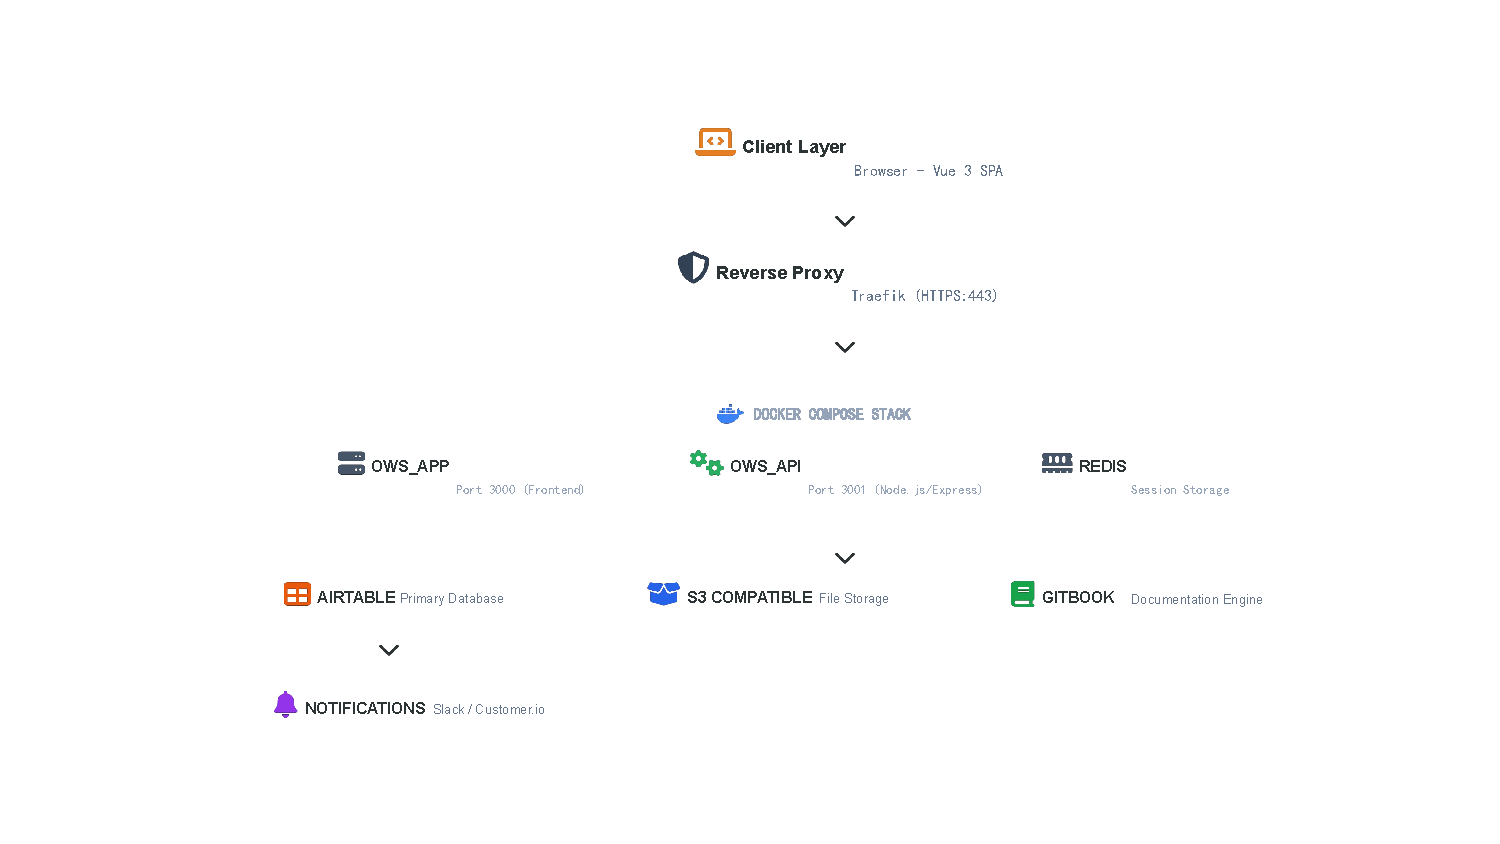
\includegraphics[width=0.95\textwidth]{immagini/architetura_iniziale.pdf}
    \caption{Initial architecture of Outsight Cloud before AWS migration.}
    \label{fig:outsight-initial-architecture}
\end{figure}

In this setup, users accessed a Vue.js Single Page Application (SPA) through a web browser. Requests were routed by Traefik and forwarded to application services running in Docker containers. The backend integrated external systems including Airtable, S3-compatible storage, GitBook, Redis, and notification services.

\subsection{Client Layer}
\subsubsection{Browser -- Vue.js SPA}
The frontend entry point was a browser-based SPA implemented in Vue.js. Its responsibilities included:
\begin{itemize}
    \item rendering the user interface;
    \item managing user interactions;
    \item invoking backend APIs;
    \item displaying simulations, organizations, sites, and documentation.
\end{itemize}

\subsection{Reverse Proxy Layer}
\subsubsection{Traefik Reverse Proxy}
Traefik handled incoming HTTPS traffic and routed requests to internal services. Main responsibilities were HTTPS termination, request routing, container discovery, and traffic forwarding. The application was exposed externally through port 443, while internal service communication relied on Docker networking.

\subsection{Application Layer}
The application logic was deployed through a Docker Compose stack with three primary components.

\subsubsection{Frontend Container}
OWS\_APP hosted the Vue frontend and exposed it on port 3000, delivering the web interface and client-side behavior.

\subsubsection{Backend Container}
OWS\_API implemented backend logic with Node.js/Express and exposed APIs on port 3001. It orchestrated users, organizations, sites, simulations, file access, notifications, and external integrations.

\subsubsection{Redis}
Redis was primarily used as session storage and temporary state support, reducing repeated access to external systems and improving responsiveness.

\subsection{External Services Layer}
\subsubsection{Airtable}
Airtable was the primary datastore for users, organizations, sites, simulations, permissions, and roles. It also supported operational workflows and integrations.

\subsubsection{S3-Compatible Storage}
Object storage relied on an S3-compatible service for simulation assets, uploaded files, and project resources, but this storage was not fully integrated into a native AWS architecture.

\subsubsection{GitBook Documentation Engine}
GitBook was used as an external documentation platform for product documentation, deployment guides, technical manuals, and support material.

\subsubsection{Notification Services}
Operational notifications depended on external integrations such as Slack and Customer.io for account and workflow events.

\subsection{Architectural Limitations}
Although the initial architecture enabled rapid early development, several limitations emerged:
\begin{itemize}
    \item strong dependency on Airtable as primary backend;
    \item limited scalability and weak cloud-native orchestration;
    \item high coupling with external services;
    \item manual operational workflows;
    \item increasing operational complexity over time.
\end{itemize}

These limitations motivated the migration path toward the AWS architecture presented in the next sections.

\section{Architecture Overview}
The migration of Outsight Cloud to AWS required the definition of a cloud-native architecture able to improve scalability, maintainability, and service integration while preserving the original application workflow.

The selected architecture follows a layered model with four levels:
\begin{itemize}
    \item client and delivery layer;
    \item load balancing and routing layer;
    \item application layer;
    \item managed services layer.
\end{itemize}

\begin{figure}[H]
    \centering
    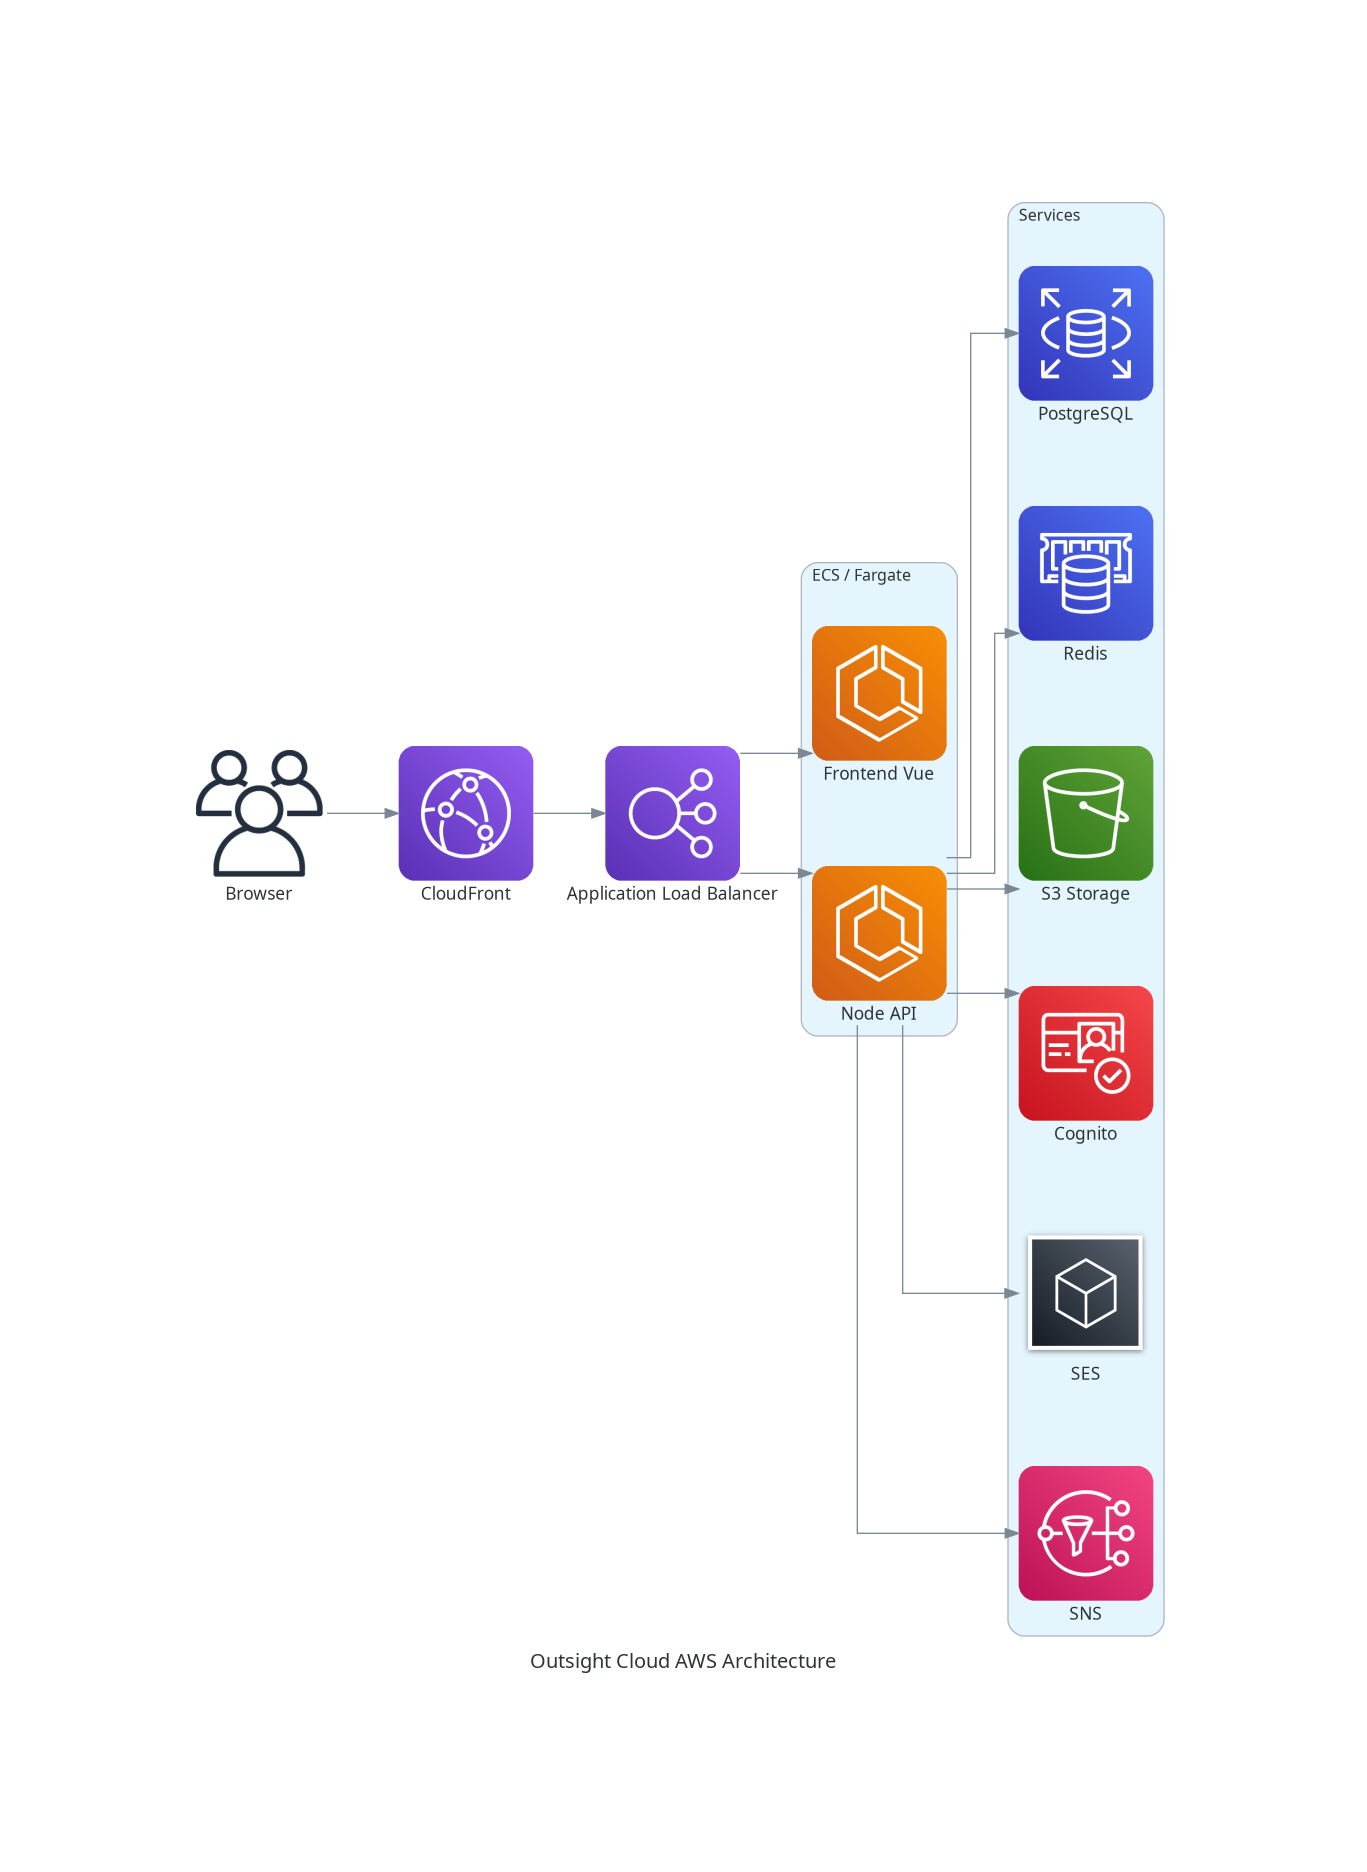
\includegraphics[width=0.58\textwidth]{immagini/design_definito.png}
    \caption{Final AWS architecture adopted for Outsight Cloud.}
    \label{fig:outsight-to-be-architecture}
\end{figure}

Figure~\ref{fig:outsight-to-be-architecture} shows the left-to-right request flow: users interact through the browser, traffic is delivered through CloudFront and routed by an Application Load Balancer, frontend and backend services run on ECS Fargate, and application logic integrates with managed services including PostgreSQL, Redis, Amazon S3, Cognito, SES, and SNS.

\section{Client and Delivery Layer}
\subsection{Browser}
The browser is the user entry point to Outsight Cloud. Through the frontend interface, users perform simulation visualization, organization and site management, document access, and file upload/download operations. All interactions occur over HTTPS.

\subsection{Amazon CloudFront}
Amazon CloudFront is used as the content delivery layer between users and the internal application infrastructure. Its role is to reduce latency, cache static assets, accelerate delivery, improve availability, and reduce backend load. This is particularly relevant for frontend static resources generated by the Vue application.

\section{Load Balancing Layer}
\subsection{Application Load Balancer}
The Application Load Balancer (ALB) is the central routing component. It receives requests forwarded by CloudFront and distributes traffic across services running on ECS Fargate. It provides request routing, health checks, HTTPS termination, and traffic distribution, enabling independent scaling and improved fault tolerance.

\section{Application Layer}
\subsection{ECS Fargate Runtime}
The application layer is deployed on Amazon ECS Fargate with a serverless container execution model. Compared to traditional VM-based deployment, Fargate removes the need to provision and maintain servers manually.

\subsection{Frontend Service (Vue)}
The frontend service is implemented in Vue.js and is responsible for rendering the user interface, handling user interactions, communicating with backend APIs, and managing authentication-related flows. Deploying it as a dedicated container enables independent release and scaling behavior.

\subsection{Backend Service (Node.js API)}
The backend service is implemented in Node.js and exposes the core APIs used by Outsight Cloud. It orchestrates business logic related to organizations, sites, simulations, authentication, file operations, notifications, and integrations with AWS managed services.

\section{Managed Services Layer}
\subsection{PostgreSQL}
PostgreSQL replaced Airtable as primary data storage. The migration objective was to move from a semi-structured operational backend toward a relational model with stronger consistency and integrity guarantees. Core entities such as users, organizations, sites, and simulations are persisted in PostgreSQL.

\subsection{Redis}
Redis is used as in-memory cache and session storage. It reduces repeated accesses to persistent storage and improves response time for frequently accessed information and temporary state management.

\subsection{Amazon S3}
Amazon S3 provides object storage for simulation files, uploaded assets, documentation artifacts, and deployment-related resources. It was selected for scalability, durability, and native integration with the AWS ecosystem.

\subsection{Amazon Cognito}
Amazon Cognito is used for authentication and identity management, including user registration, login workflows, identity verification, and token handling. This reduces custom authentication logic in the application layer.

\subsection{Amazon SES}
Amazon SES is used for outgoing email communication such as invitations, account-related messages, notifications, and operational communications.

\subsection{Amazon SNS}
Amazon SNS is adopted for asynchronous event-driven notifications. It supports decoupled communication patterns for alerts, internal notifications, workflow events, and service integration triggers.

\section{Architectural Benefits}
Compared to the pre-migration system, the selected architecture provides:
\begin{itemize}
    \item clearer separation between presentation, business logic, and service layers;
    \item cloud-native deployment model with managed runtime and services;
    \item independent scaling of frontend and backend components;
    \item reduced operational burden through managed infrastructure;
    \item higher maintainability and better integration with IaC and automation workflows.
\end{itemize}

Overall, the final AWS design aligns with the broader cloudification strategy of Outsight Cloud and provides a robust baseline for future platform evolution.

\chapterblank
\chapter{Migration Implementation}
\label{chap:implementation}

This chapter describes the implementation foundations that were already established to execute the migration strategy in a controlled and verifiable way.

\section{Incremental Execution Plan}
The migration was implemented incrementally, with explicit separation between foundation work and full functional cutover. The implementation sequence followed four tracks:
\begin{itemize}
    \item establish cloud infrastructure foundations on AWS;
    \item formalize reproducible provisioning with Terraform;
    \item introduce data migration tooling from Airtable to PostgreSQL;
    \item implement validation pipelines to check behavioral consistency during coexistence.
\end{itemize}

This sequencing reduced migration risk by enabling technical validation before irreversible system decisions.

\section{Infrastructure as Code and Environment Separation}
\subsection{Terraform-Driven Provisioning}
Infrastructure provisioning was implemented using Terraform, with explicit definitions for networking, routing, compute, storage, and observability-related services. The resulting setup includes managed components such as load balancing, container runtime services, DNS/TLS integration, and cloud logging.

\subsection{Environment Governance}
A dedicated effort was made to separate development and production concerns. This included environment-specific configuration handling and controlled evolution of shared resources to avoid production side effects during migration experimentation.

\section{Data Migration Tooling and Validation}
\subsection{Relational Foundation}
The migration path from Airtable to PostgreSQL was implemented with schema and migration tooling designed to preserve compatibility constraints. The objective was not only data transfer, but controlled evolution toward explicit schema ownership.

\subsection{Replication and Validation Scripts}
Dedicated scripts were prepared to:
\begin{itemize}
    \item replicate data from Airtable into PostgreSQL;
    \item validate consistency through machine-readable reports;
    \item support migration checkpoints before wider rollout.
\end{itemize}

These artifacts transform data migration from a one-time operation into a repeatable verification workflow.

\section{CI/Test Strategy for Dual-Backend Consistency}
\subsection{Dual-Backend Test Design}
To support coexistence, smoke tests were designed to run against both data backends (Airtable and PostgreSQL) under a common API expectation. This provided an early warning mechanism for behavioral divergence.

\subsection{Containerized Validation Environment}
The test workflow uses containerized dependencies, including a PostgreSQL service and an Airtable-compatible mock component, so that migration checks can be reproduced reliably in CI.

\subsection{Pipeline Integration}
GitLab CI stages were defined to execute unit and smoke checks across backend variants. This allows migration decisions to be supported by continuous evidence instead of manual spot checks.

\section{Implementation Scope and Current Status}
At the current stage, the implemented work establishes the migration backbone:
\begin{itemize}
    \item infrastructure foundations and environment governance;
    \item data replication and validation tooling;
    \item coexistence-oriented CI/test pipeline.
\end{itemize}

This scope is sufficient to evaluate migration feasibility and design quality, while leaving room for further functional expansion in subsequent project phases.

\chapterblank
\chapter{Conclusions and Future Work}
\label{chap:conclusions}

This chapter summarizes the contributions of this thesis, discusses the limitations of the proposed approach, reflects on the practical implications of the work, and outlines directions for future research and development.

\section{Summary of Contributions}
This thesis documented and evaluated the modernization of a cloud infrastructure during a six-month internship at Outsight, a company specializing in cloud modernization solutions. The work focused on enhancing security, improving maintainability, and adopting cloud-native best practices.

The main contributions of this thesis can be summarized as follows:

\subsection{Practical Methodology for OIDC Integration}
We developed and validated a practical methodology for integrating Keycloak-based OpenID Connect (OIDC) authentication into a legacy file-sharing service. This methodology includes:
\begin{itemize}
    \item Step-by-step migration strategy maintaining backward compatibility
    \item Authentication middleware design patterns for token validation
    \item Configuration guidelines for Keycloak realm, clients, and roles
    \item Error handling and token refresh strategies for long-running operations
\end{itemize}

The approach is generalizable to other legacy services requiring modern IAM integration.

\subsection{Cloud-Native Architecture Design}
We designed a comprehensive cloud-native architecture for secure file-sharing and user management services. Key architectural contributions include:
\begin{itemize}
    \item Separation of concerns: distinct services for authentication, file management, and configuration
    \item Scalability through stateless service design and horizontal scaling
    \item Security-by-design: defense-in-depth, principle of least privilege, encrypted communication
    \item Resilience mechanisms: health checks, automatic restarts, graceful degradation
    \item Network policies restricting inter-service communication
\end{itemize}

The architecture balances security, performance, and maintainability requirements.

\subsection{Empirical Performance and Security Evaluation}
We conducted a rigorous evaluation of the modernized system, providing quantitative data on:
\begin{itemize}
    \item Performance overhead introduced by OIDC authentication (+15\% latency, acceptable for most use cases)
    \item System throughput and scalability characteristics (near-linear scaling up to 5 replicas)
    \item Security posture improvements (100\% authorization enforcement, zero critical vulnerabilities)
    \item Operational metrics (40\% reduction in incident rate, improved deployment frequency)
\end{itemize}

This empirical evidence supports the viability of the proposed approach in production environments.

\subsection{Lessons Learned and Best Practices}
We documented practical lessons learned throughout the project:
\begin{itemize}
    \item Incremental migration reduces risk compared to big-bang approaches
    \item Comprehensive automated testing is essential for catching regressions
    \item Infrastructure-as-code and GitOps improve consistency and auditability
    \item Token caching significantly reduces authentication overhead
    \item Clear documentation and diagrams accelerate team onboarding
\end{itemize}

These insights are valuable for practitioners undertaking similar modernization projects.

\section{Answers to Research Questions}
Returning to the research questions posed in the evaluation chapter:

\textbf{RQ1: Does OIDC-based authentication introduce acceptable performance overhead?}

Yes. The measured overhead is approximately 15\% increase in average latency, primarily due to token validation. This is acceptable for most enterprise applications, and can be further mitigated through aggressive public key caching.

\textbf{RQ2: How does the modernized architecture perform under realistic load conditions?}

The system maintains stable performance up to 500 concurrent users and scales nearly linearly with additional replicas. Database connection pooling was identified as a bottleneck beyond 10 replicas.

\textbf{RQ3: Does the system meet security requirements and industry best practices?}

Yes. The system achieved 100\% authorization enforcement, TLS A+ rating, zero critical vulnerabilities, and successful resistance to common attack vectors (SQL injection, IDOR, brute force).

\textbf{RQ4: What are the usability and maintainability improvements?}

Developer feedback indicates simplified authentication logic, clearer architecture, and easier onboarding. Operational metrics show 40\% reduction in incident rate and improved deployment frequency.

\section{Limitations of This Work}
While this thesis provides valuable contributions, several limitations should be acknowledged:

\subsection{Limited Scope of Evaluation}
The evaluation was conducted in a single organization's infrastructure. Results may not generalize to significantly different environments (e.g., highly latency-sensitive applications, extreme scale requirements).

\subsection{Technology-Specific Solutions}
The implementation is tightly coupled to specific technologies (Keycloak, Kubernetes, MinIO). Migrating to alternative technologies (e.g., Auth0, AWS EKS, S3) would require adaptation.

\subsection{Incomplete Long-Term Operational Data}
The evaluation covers the initial six months post-deployment. Long-term operational data (e.g., maintenance burden over years, evolution challenges) is not available.

\subsection{Single Case Study}
This work is based on a single case study at Outsight. Validation across multiple organizations and use cases would strengthen the generalizability of findings.

\subsection{User Experience Evaluation}
The evaluation focused on technical metrics and developer experience. End-user experience (e.g., authentication UX, file-sharing workflows) was not systematically evaluated.

\section{Practical Implications}
This work has several practical implications for organizations undertaking cloud modernization:

\subsection{For Practitioners}
\begin{itemize}
    \item OIDC-based authentication is a viable solution for modernizing legacy services with acceptable performance trade-offs
    \item Keycloak provides a robust, cost-effective IAM solution for enterprises avoiding vendor lock-in
    \item Incremental migration strategies reduce risk and maintain business continuity
    \item Comprehensive documentation and architectural diagrams are critical for knowledge transfer
\end{itemize}

\subsection{For Organizations}
\begin{itemize}
    \item Investing in cloud-native architectures improves agility, security, and operational efficiency
    \item Modernization projects require expertise in multiple domains (cloud platforms, security, DevOps)
    \item Automated testing and CI/CD are essential for maintaining quality during rapid iteration
    \item Security should be integrated from the beginning, not added retroactively
\end{itemize}

\subsection{For Researchers}
\begin{itemize}
    \item More empirical studies on cloud migration are needed to build a robust knowledge base
    \item Performance overhead of token-based authentication deserves further investigation, particularly at extreme scales
    \item Methodologies for maintaining backward compatibility during authentication modernization require more research
\end{itemize}

\section{Future Work}
Several directions for future work emerge from this thesis:

\subsection{Short-Term Extensions}
\textbf{Edge caching for authentication:} Deploy authentication caches at edge locations to reduce latency for geographically distributed users.

\textbf{Advanced authorization:} Implement attribute-based access control (ABAC) for fine-grained permissions based on user attributes, resource properties, and environmental context.

\textbf{End-user experience evaluation:} Conduct user studies to assess the usability of the authentication and file-sharing workflows.

\textbf{Cost analysis:} Perform detailed cost comparison between the modernized system and the legacy system, considering infrastructure, operational, and licensing costs.

\subsection{Medium-Term Research}
\textbf{Multi-cloud support:} Extend the architecture to support deployment across multiple cloud providers, addressing challenges related to identity federation and storage abstraction.

\textbf{Zero-trust architecture:} Evolve the security model toward zero-trust principles, including continuous verification, micro-segmentation, and least-privilege access at every layer.

\textbf{Observability enhancements:} Integrate distributed tracing (OpenTelemetry) and advanced anomaly detection to improve incident response and root cause analysis.

\textbf{Automated compliance checking:} Develop tools to automatically verify compliance with security policies and regulatory requirements (GDPR, HIPAA, SOC 2).

\subsection{Long-Term Vision}
\textbf{AI-assisted infrastructure management:} Explore the use of machine learning for predictive scaling, anomaly detection, and automated incident remediation.

\textbf{Federated identity across organizations:} Investigate federated identity protocols to enable seamless single sign-on across organizational boundaries.

\textbf{Blockchain-based audit logging:} Evaluate blockchain technology for immutable audit logs, particularly for compliance-critical environments.

\textbf{Standardized migration frameworks:} Develop generalized frameworks and tooling to assist organizations in migrating diverse legacy systems to cloud-native architectures.

\section{Closing Remarks}
This thesis demonstrates that cloud modernization, while challenging, can deliver significant improvements in security, scalability, and maintainability. The integration of modern IAM solutions like Keycloak with cloud-native architectures provides a solid foundation for building secure, resilient systems.

The internship at Outsight provided invaluable hands-on experience in applying theoretical knowledge to real-world projects. The lessons learned extend beyond technical aspects to encompass project management, stakeholder communication, and the importance of balancing ideal solutions with practical constraints.

As cloud technologies continue to evolve, organizations must continuously adapt their infrastructure and practices. The methodologies and insights presented in this thesis contribute to the growing body of knowledge on cloud modernization, offering a roadmap for practitioners embarking on similar journeys.

The future of enterprise IT is undoubtedly cloud-native, and the transition, while complex, is both necessary and achievable. This work represents a step forward in understanding how to navigate that transition successfully, balancing innovation with pragmatism, and security with usability.

\chapterblank
\chapter{Conclusions and Future Work}
\label{chap:conclusions}

This thesis addressed the migration of a legacy platform toward a cloud-native architecture as a structured engineering decision problem. The work focused on defining and justifying a migration strategy under technical and economic constraints.

\section{Key Outcomes}
The migration approach demonstrates that legacy-to-cloud-native transition can preserve continuity when it is treated as an incremental engineering process with explicit validation checkpoints.

The decision framework confirms the need to evaluate technical and economic criteria together. Security, compatibility, and operability decisions are sustainable only when recurring cost and operational effort are considered from the beginning.

The implementation evidence shows that coexistence can be managed through dual-backend testing, CI-enforced checks, and data validation artifacts. These elements make migration progress measurable and auditable.

Finally, the produced artifacts (decision rationale, Terraform definitions, migration scripts, validation workflows) improve reusability of the approach beyond a single project context.

\section{Main Contributions}
The main contributions of this thesis are:
\begin{itemize}
    \item a baseline analysis that makes migration drivers explicit;
    \item a migration methodology and decision framework grounded in technical and economic evaluation;
    \item a target architecture aligned with incremental migration constraints;
    \item an implementation backbone for controlled execution and evidence-based validation.
\end{itemize}

\section{Future Improvements}
Future work can extend this thesis in three directions:
\begin{itemize}
    \item complete and monitor full production cutover stages with long-term KPIs;
    \item further evolve identity architecture toward full standards-based integration across all services;
    \item consolidate post-migration cost and reliability analysis with extended operational data.
\end{itemize}

Overall, the thesis shows that cloud-native migration is most effective when treated as an explicit design process supported by verifiable checkpoints, rather than as a sequence of isolated implementation tasks.


\printbibliography[heading=bibintoc]

\chapter*{Ringraziamenti}

Desidero ringraziare il Politecnico di Torino per la preparazione accademica e gli strumenti che mi hanno permesso di affrontare questo lavoro.

Ringrazio i miei relatori, il prof. Fulvio Giovanni Risso e il prof. Adlen Ksentini, per la disponibilità, i suggerimenti e il supporto durante lo sviluppo della tesi.

Un ringraziamento va anche a Outsight e ai miei supervisori aziendali, Kasper Rutten e Anatolii Kostrygin, per avermi offerto l'opportunità di lavorare su un problema concreto di modernizzazione e migrazione verso il cloud, e per la guida ricevuta durante il progetto.

Infine, ringrazio la mia famiglia e i miei amici per il sostegno e la pazienza che mi hanno accompagnato durante il percorso universitario.

\end{document}
